\chapter{Background and Motivation}

In this chapter we summarize the background and motivation underlying this work. In Section \ref{sec:bm_smt}, we briefly review the approaches to machine translation (MT) and the comparison between them.

Section \ref{sec:bm_nmt} reviews the formulation of MT in neural network as well as the frameworks utilized to solve the problem.

Section \ref{sec:weight_init} provides the definition of weight initialization in deep neural network and the importance of finding the right initialization to be able to gain an optimum performance.

Section \ref{sec:bm_tl} discuss transfer learning (TL) as well as its variants.

Finally, Section \ref{sec:bm_adapters} discuss adapters module as an alternative methodology in fine-tuning the model and provides reasons, why we focus our research by using adapters.

\section{Machine Translation}
\label{sec:bm_smt}
On a fundamental level, MT performs substitution of words from one language to the other. However, it is difficult to produce a good translation based on the substitution alone as understanding the whole sentence that includes phrases and surrounding words in the target language is needed. The problem is exacerbated as words may have more than one meaning and it is difficult to determine one-to-one relation in another language.

There are three main approaches in MT that most commonly used: rule-based, statistical (SMT) and neural (NMT). Due to the effort of manual collection of good dictionary and grammatical rules, demands on automatic approach such as SMT or NMT seems more appealing.
Prior to NMT, a variant of SMT namely phrase-based machine translation (PBMT) had been the state-of-the-art for German-to-English language pairs. \cite{bojar2015proceeding} also shows that PBMT have a good performance in different language pairs. \cite{blunsom2013recurrent} introduced the first end-to-end neural network for machine translation with encoder-decoder structure. Their approach encodes a given source text into a continuous vector and further transform the state vector into the target language.

While NMT has been the main technique used in various MT challenges such as WMT, there are some advantages and disadvantages. According to \cite{koehn2017nmt}, NMT suffers from the following phenomenon:
\begin{itemize}
    \item In out-of-domain scenario, NMT systems have a lower quality. The author found that the model completely sacrifice adequacy over fluency
    \item NMT requires a large amount of data. This is problematic when low-resource languages are involved in the evaluation.
    \item NMT does not perform well in low-frequency words. PBMT performance suffers when the low-frequency words occur in the sentence. This is especially true when the word is completely unknown. Although NMT better performed in a low-frequency words, the problem is not yet solved. From the experiments, the NMT models also show weakness in translating low-frequency words.
    \item Problem in translating long sentences. NMT can performs well in short sentences up to 60 words. However, for longer sentences it shows lower quality of translation.
    \item Model interpretability. As opposed to PBMT, it is difficult to interpret the behaviour of NMT due to the complexity introduced in the hyperparameter as well as the model architecture. Furthermore, the training of NMT also non-deterministic due to random parameter initialization.
\end{itemize}

Despite its shortcomings, NMT also shows promising direction in MT. (\cite{machavcek2018enriching}) mentioned that the difference is apparent in the output fluency. They mentioned PBMT models suffer from problems such as double negation and translation morphologically rich languages. These problems cause little to no problem at all in NMT models.

\section{Neural Machine Translation}
\label{sec:bm_nmt}
We define the translation problem as a mapping function $t$ of sentences from a given source language $S$ and target language $T$ from parallel corpus, where $t : S \rightarrow T$. The definition of parallel corpus is a pair of sentences in two different languages where one sentence in $T$ corresponds to its equivalent in language $S$. The goal of function $t$ is to find the highest probability of word $y \in T$ from $x \in S$, where $t(x) = argmax_y(p(y|x))$. The probability $p(y|x)$ is the probability estimation given by the NMT model.

In the following sections, we show a quick overview of recent NMT models, this includes their architecture, advantages, and their drawbacks.

\subsection{RNN Seq2Seq}
The first seq2seq model that employs RNN as the fundamental architecture is proposed by \cite{sutskever2014sequence}. This is a straightfoward extension from language model problem. Essentially, the model sequentially predict the next word given all previous words.

In MT, the approach is modified by using two similar model architectures for language $S$ and $T$. For language $S$ we call this component \texttt{encoder} and for $T$ we call it \texttt{decoder}.
The task of \texttt{encoder} is to produce a vector representation of the input sentence from source language $x \in S$. We define the input sentence as a sequence of tokens from a fixed set of vocabulary $x \in S$ that transformed by an embedding matrix containing dense representation. These representation is then processed by an RNN. This results in a new representation for each tokens encoded by hidden states in RNN. This representation can be think of as a combination of features from the token and its context.
\texttt{decoder} has a similar functionality as \texttt{encoder} where it uses a sequence of tokens from $y \in T$ as its inputs. \texttt{decoder} leverage additional features from \texttt{encoder} by incorporating the output vector of \texttt{encoder}. The output vector from \texttt{encoder} represents the final token of the sentence. For further illustration, we refer to Image \ref{img:rnnseq2seq}.

\begin{figure}[h]
    {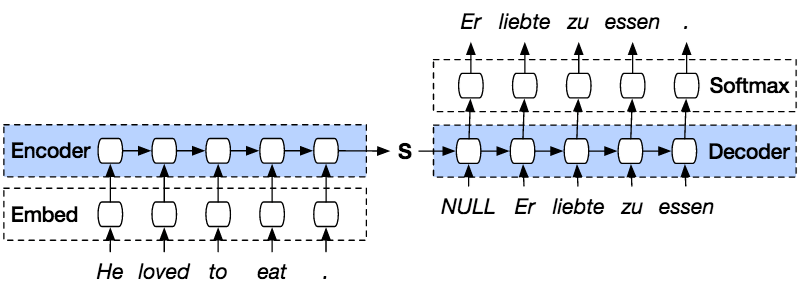
\includegraphics[width=0.95\textwidth]{img/rnnseq2seq.png}}
    \centering
    \caption{Illustration of seq2seq architecture. Figure reprinted from \protect\url{https://www.guru99.com/seq2seq-model.html}.}
    \label{img:rnnseq2seq}
\end{figure}

The disadvantages of this model is found by \cite{cho2014properties}. They found that the models performance decreases when the length of source sentence increased. We recall that the only features used by the \texttt{decoder} to refer to the original source sentence is through the last token vector from the \texttt{encoder}. The vector is a fixed-size vector where the length is pre-defined prior to the training. In essence, this vector tries to combine the features from all the words in the original source sentence. Hence, when the source sentence grow, the vector could potentially be less informative due to the more information it has to encode.

Furthermore, RNNs also suffer in the problem where the gradient can be extremely small or large. These problems are often mentioned as vanishing and exploding gradient problem. When the gradient of the model is extremely small, RNNs can not learn from the data effectively, especially in the long-range dependencies setup. On the other hand, when the gradient is extremely large, it can affect the weight parameters by moving them far away from the optimal space. This would distrupt the learning process and can cause the model fail to learn. This problem can happen in seq2seq architecture as we esssentially backpropagate the weights from the end of the \texttt{decoder} to the beginning of the \texttt{encoder}.

\subsection{Seq2Seq with Attention}
In order to address the aforementioned issue, (\cite{bahdanau2015nmt}) introduce an extension to the encoder-decoder model which learns
to align and translate jointly. Each time the proposed model generates a word in a translation, it
(soft-)searches for a set of positions in a source sentence where the most relevant information is
concentrated. The model then predicts a target word based on the context vectors associated with
these source positions and all the previous generated target words.

\begin{figure}[h]
    {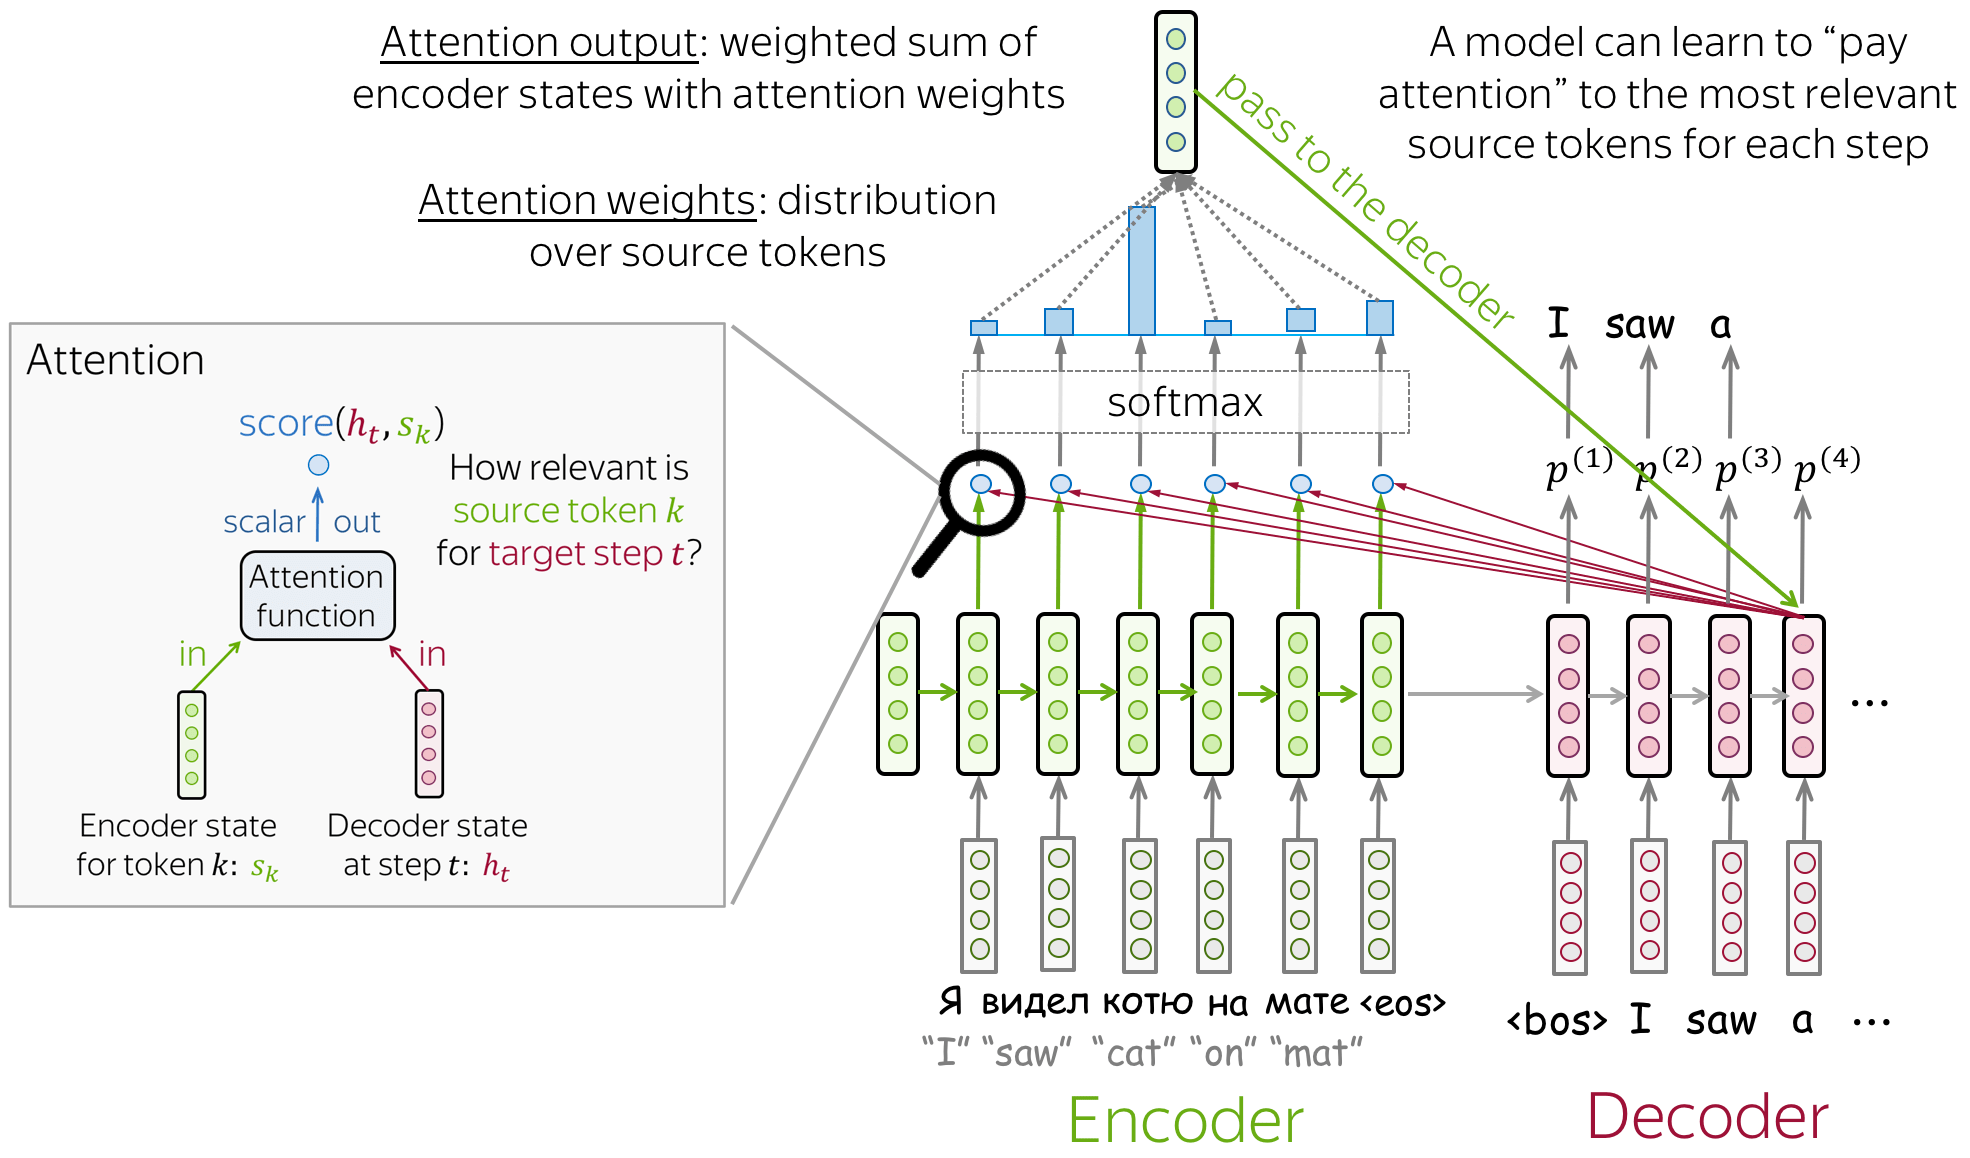
\includegraphics[width=0.95\textwidth]{img/attseq2seq.png}}
    \centering
    \caption{Illustration of seq2seq architecture with attention. Figure reprinted from \protect\url{https://lena-voita.github.io/nlp_course/seq2seq_and_attention.html}.}
    \label{img:attseq2seq}
\end{figure}

The most important distinguishing feature of this approach from the basic encoder-decoder is that
it does not attempt to encode a whole input sentence into a single fixed-length vector. Instead, it encodes the input sentence into a sequence of vectors and chooses a subset of these vectors adaptively
while decoding the translation. This frees a neural translation model from having to squash all the
information of a source sentence, regardless of its length, into a fixed-length vector. We show this
allows a model to cope better with long sentences.

show that the proposed approach of jointly learning to align and translate achieves
significantly improved translation performance over the basic encoder-decoder approach. The im-
provement is more apparent with longer sentences, but can be observed with sentences of any
length. On the task of English-to-French translation, the proposed approach achieves, with a single
model, a translation performance comparable, or close, to the conventional phrase-based system.

The motivation is that we want to compute an association between the decoder state (which
contains information where we are in the output sentence production) and each input word.
Based on how strong this association is, or in other words how relevant each particular input
word is to produce the next output word, we want to weight the impact of its word represen-
tation. We can see the illustration of this architecture from Figure \ref{img:attseq2seq}

\subsection{Transformer}
Recurrent models typically factor computation along the symbol positions of the input and output
sequences. Aligning the positions to steps in computation time, they generate a sequence of hidden
states ht, as a function of the previous hidden state $h_{t-1}$ and the input for position t. This inherently
sequential nature precludes parallelization within training examples, which becomes critical at longer
sequence lengths, as memory constraints limit batching across examples. Recent work has achieved
significant improvements in computational efficiency through factorization tricks and conditional
computation, while also improving model performance in case of the latter. The fundamental
constraint of sequential computation, however, remains

Figure \ref{img:transformer} illustrates the Transformer architecture. The left part is the en- coder, the right is part is the decoder. One attention component is inside the encoder. It assigns to each word an attention score of every other word in the sen- tence. The authors claim3 that this module is able to solve coreference between any pair of words in single step, while sequential models need a higher number of steps to transport the information to corresponding positions in sequence, and thus performs slower and worse. Another attention module is inside the decoder and on the boundary between the encoder and decoder.

(\cite{vaswani2017attention}) show experiments that the Transformer architecture outperformed previous model with much lower training cost. In their blogpost,3 the authors claim (without further details) that the same network they used for English to German translation, with a little adaptation, outperformed all but one of the previously proposed approaches to constituency parsing.

\begin{figure}[h]
    {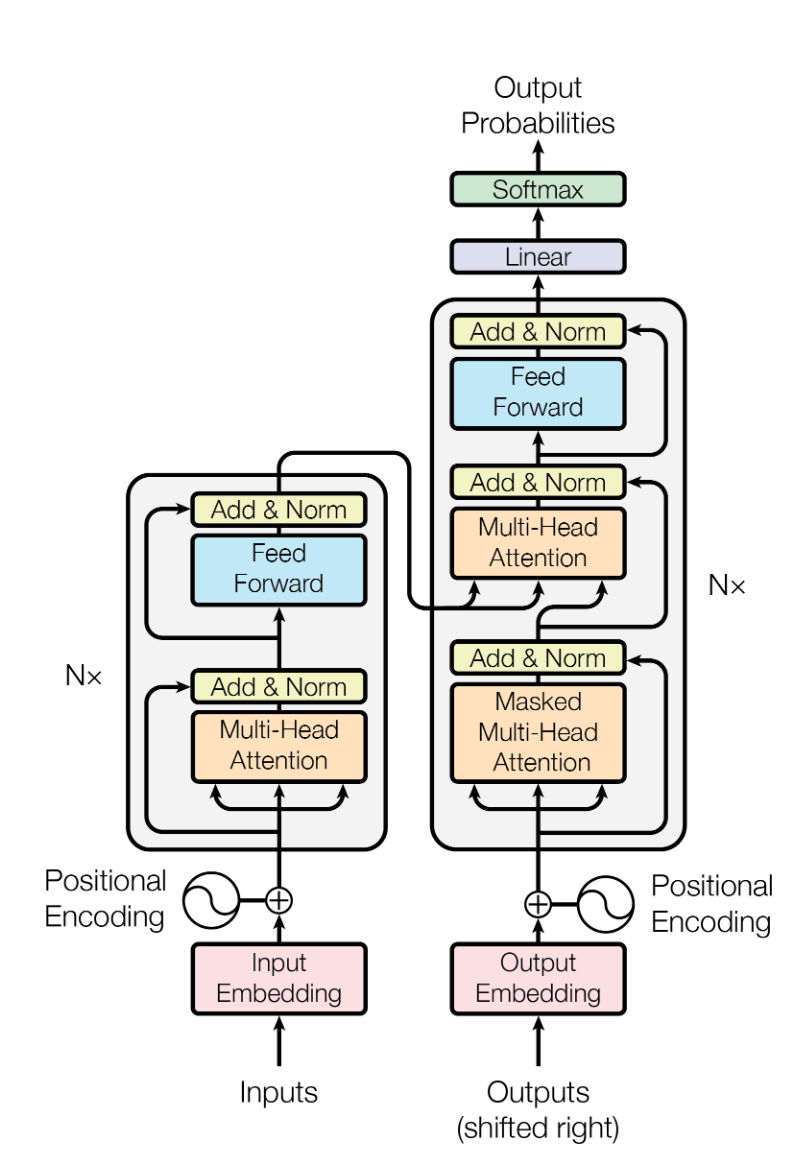
\includegraphics[width=0.75\textwidth]{img/transformer.png}}
    \centering
    \caption{Illustration of Transformer model. Figure reprinted from \cite{vaswani2017attention}.}
    \label{img:transformer}
\end{figure}

Based on \cite{liu2020understanding}, despite its contribution in leading many breakthroughs in NLP space, transformer requires non-trivial efforts in training the models. In contrary to other neural layers such as recurrent neural network (RNN) and convolution neural network (CNN), optimization such as stochastic gradient descent (SGD) may converge to bad/suspicious local optima if not tuned carefully. Furthremore, the warmup stage is crucial during the training as removing them leads to severe consequences such as model divergence. From this finding, we understand that training Transformer and obtaining an optimal performance is not really straightforward.

\section{Weights Initialization}
\label{sec:weight_init}
The aim of weight initialization is to prevent layer activation outputs from exploding or vanishing during the course of a forward pass through a deep neural network. If either occurs, loss gradients will either be too large or too small to flow backwards beneficially, and the network will take longer to converge, if it is even able to do so at all.

Matrix multiplication is the essential math operation of a neural network. In deep neural nets with several layers, one forward pass simply entails performing consecutive matrix multiplications at each layer, between that layer's inputs and weight matrix. The product of this multiplication at one layer becomes the inputs of the subsequent layer, and so on and so forth.

Most of the recent experimental results with deep architecture are obtained with models that can be turned into deep supervised neural networks, but with initialization or training schemes different from the classical feedforward neural networks (Rumelhart et al., 1986). Why are these new algorithms working so much better than the standard random initialization and gradient-based optimization of a supervised training criterion? Part of the answer may be found in recent analyses of the effect of unsupervised pretraining (\cite{erhan2009thedifficulty}), showing that it acts as a regularizer that initializes the parameters in a “better” basin of attraction of the optimization procedure, corresponding to an apparent local minimum associated with better generalization.

\begin{figure}[h]
    {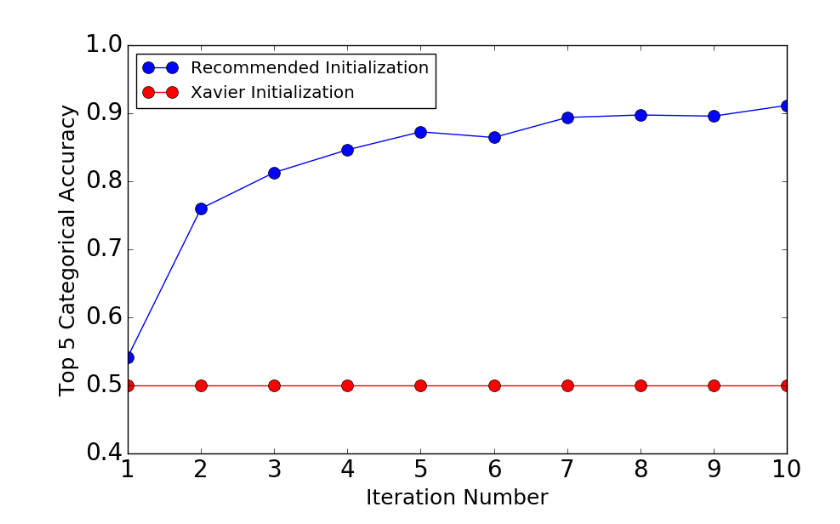
\includegraphics[width=0.95\textwidth]{img/comp_init.png}}
    \centering
    \caption{Comparison of neural network performance using different initialization technique. Figure reprinted from \cite{kumar2017onweight}.}
    \label{img:comp_init}
\end{figure}

To show the impact of good initialization, we refer to the work of \cite{kumar2017onweight}. In this work, the author provides a recommendation to initialize a neural network with sigmoid activation function. The experiment was done in Computer Vision area using CIFAR10 dataset. The author compares the result of the initialization with one of the most used initialization such as Xavier initialization (\cite{glorot2010understanding}). The result of the experiment can be seen at \ref{img:comp_init}. We can see from this graph the gap between different initialization is quite apparent.

\section{Transfer Learning}
\label{sec:bm_tl}
Transfer learning (TL) is a research problem in machine learning (ML) that focuses on storing knowledge gained while solving one problem and applying it to a different but related problem.
The general definition of transfer learning is given a source domain $D_S$ and learning task $T_S$, a target domain $D_T$ and learning task $T_T$, where $D_S \neq D_T$, or $T_S \neq T_T$, transfer learning aims to help improve the learning of the target predictive function $f_{T}(\cdot)$ in $D_T$ using the knowledge in $D_S$ and $T_S$. For better illustration on TL, we can refer to Figure \ref{img:transfer_learning}

\begin{figure}[h]
    {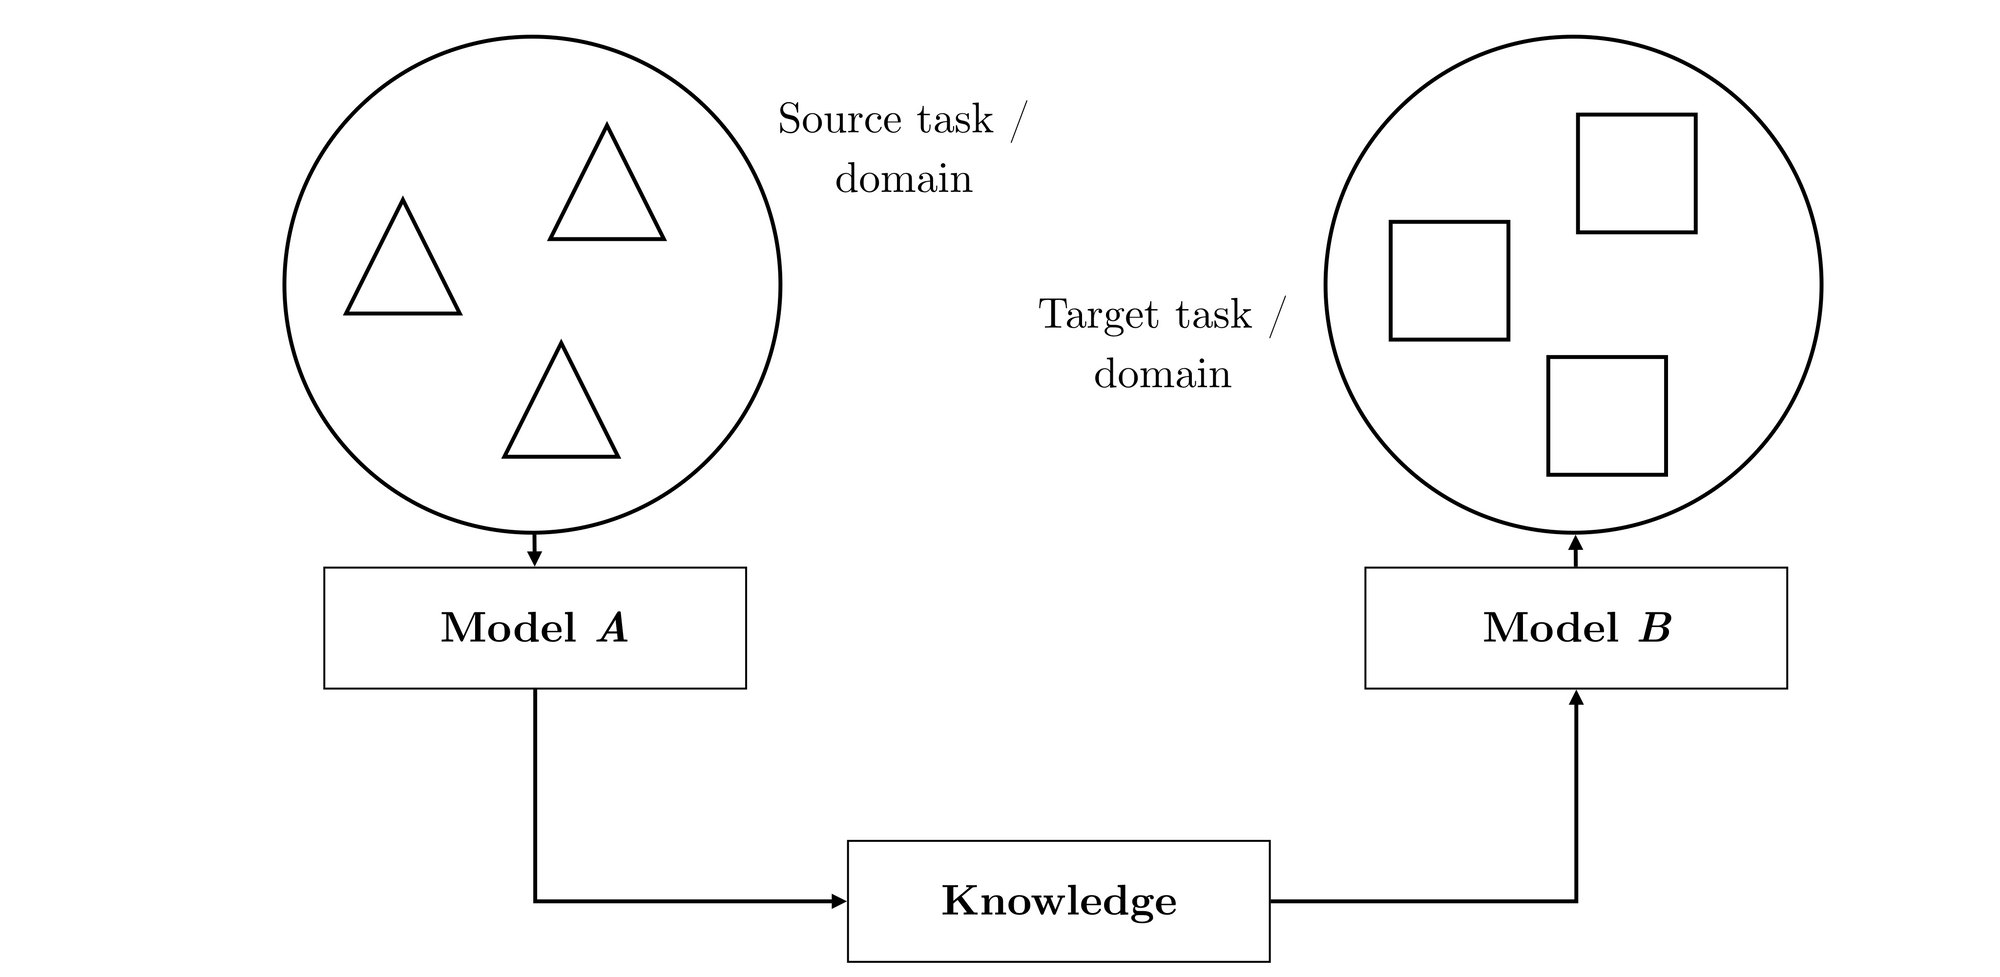
\includegraphics[width=0.95\textwidth]{img/transfer_learning_scenario.png}}
    \centering
    \caption{An illustration of transfer learning in different domain. Figure reprinted from \cite{ruder2019transfer}.}
    \label{img:transfer_learning}
\end{figure}

\cite{shavlik2010transfer} describe three ways of how transfer learning can
improve performance. Specifically:
\begin{itemize}
    \item improving the initial performance at the beginning of training compared
          to a randomly initialized model when the tasks are similar;
    \item shortening the time needed to reach the maximal performance;
    \item improving the final performance level compared to training the model
          without the transfer
\end{itemize}

To some extent, we can see TL as a way to initialize neural network with more constraints than the usual definition of weights initialization. In weight initializations, we focus on initializing random weights for any type of neural network architecture. On the other hand, TL only applicable to a specific parts of the neural network architecture within the same domain problem. Domain problem can be defined as a category of cognitive problems such as Computer Vision, Natural Language Processing, or Speech Recognition. As of this writing, we are not aware of any algorithm to perform transfer learning in different domain category.

For this work, we are specifically interested in two of the following categories of TL: 1) Domain adaptation; 2) Sequential transfer learning. On the next sections, we will discuss the difference between these two categories.

\subsection{Domain Adaptation}
In the context of NMT, we can distinguish two categories of transfer learning. The first category is domain adaptation where we are dealing with the same language pairs but in different domain. For example, we pre-train a model in WMT data in German$\rightarrow$English pair and perform an adaptation in IWSLT data within the same language. On the second category, we have multilingual adaptation. In this category we are dealing with completely different language pairs between the pre-training and the fine-tuning. For the scope of this project, we limit the problem into domain adaptation.

Domain adaptation is one of the critical issues in MT, where the goal is to specialize the model for a more specific domain. It is well known that an optimized model on a specific genre (news, speech, medical, literature, and other) obtains higher accuracy results than a generic system on the given domain (\cite{gao2002improving,hildebrand2005adaptation}). Specifically, when the training data have an unbiased distribution over the target domain, the final model will perform comparably on testing data as it performed during training on the development set. However, the performance will decrease if the training data comes from a different domain than the target domain (see Section 2.1.1). For example, when the training data are from news articles and the test domain is more specific as medical. Domain adaptation generally encompasses terminology, domain, and style adaptation.

In a typical NMT domain adaptation setup (\cite{luong2015stanford,Servan2016DomainSA,Chu2018ASO}), we first train a parent model on a resource-rich out-of-domain parallel corpus. After the model is trained on the general model, we exchange the training corpus for the in-domain one and follow by fine-tuning the parent model. We can view the domain adaptation as transfer learning from the out-of-domain parent model into the domain-specific child model.

\cite{Freitag2016FastDA} stated two problems of domain adaptation. First, it is prone to over-fitting due to the limited amount of in-domain data. Second, the process of fine-tuning the parent model on the in-domain data leads to deteriorating the performance on the general domain. \cite{Freitag2016FastDA} propose to tackle the problem by ensembling the parent model with the child model. They showed that the ensembled model improves on the in-domain testset and preserves its performance on the general domain. \cite{Chu2017AnEC} address these problems by mixed fine-tuning, where they combine the out-of-domain corpus with oversampled in-domain data before adapting the general model.

\subsection{Sequential Transfer Learning}
Sequential transfer learning is the form that has led to the biggest improvements so far. The general practice is to pretrain representations on a large unlabelled text corpus using your method of choice and then to adapt these representations to a supervised target task using labelled data as can be seen below. For better illustration, we refer to Figure \ref{img:seq_tl}

\begin{figure}[h]
    {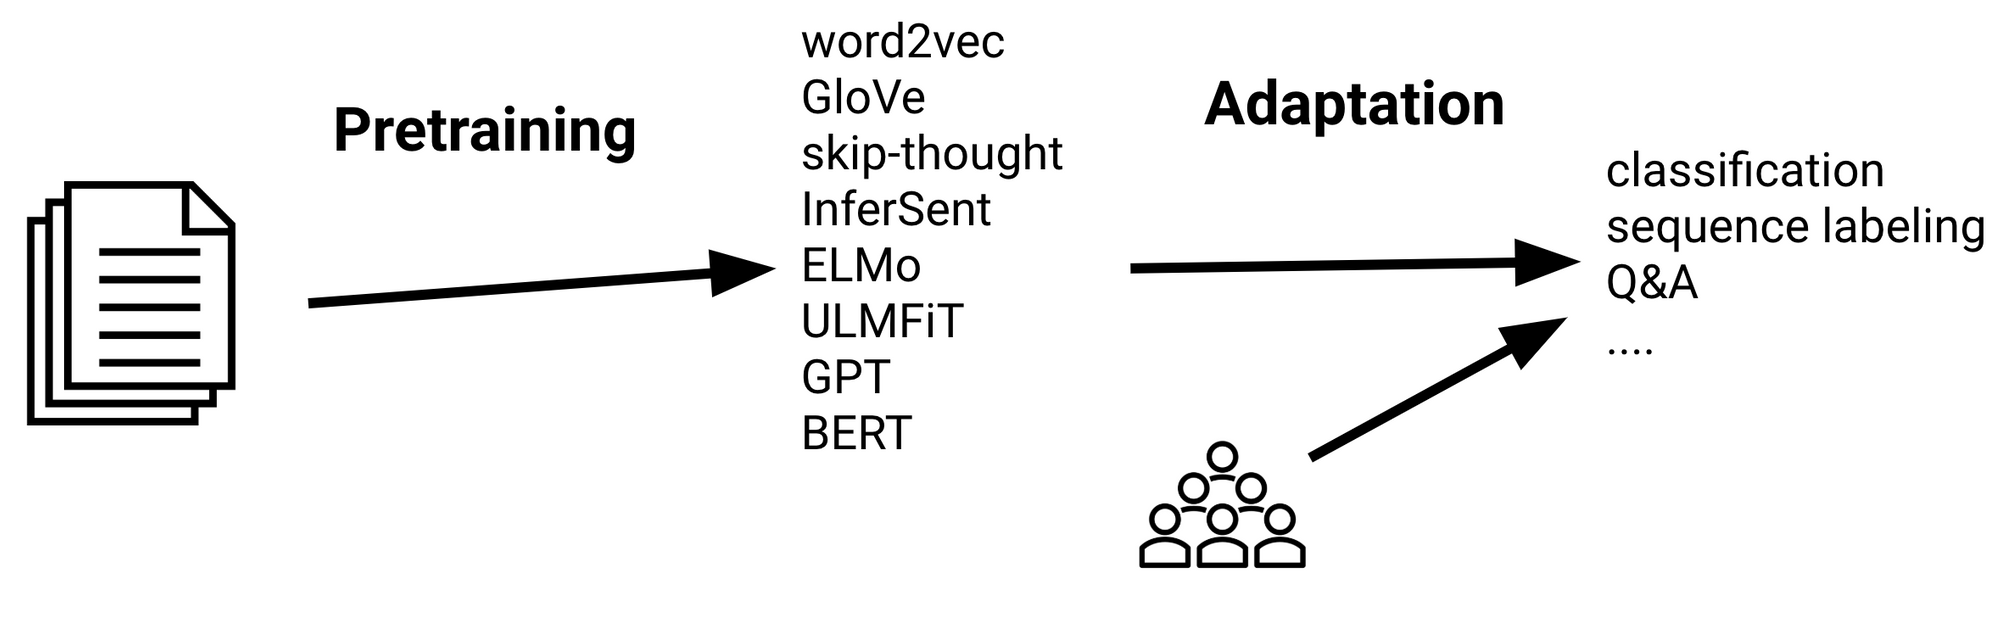
\includegraphics[width=0.95\textwidth]{img/sequential_tl.png}}
    \centering
    \caption{Illustration of sequential transfer learning. Figure reprinted from \cite{ruder2019transfer}.}
    \label{img:seq_tl}
\end{figure}

One of the most prominent examples of sequential transfer learning is language model pre-training.
Language model pre-training has been shown to be effective for improving many natural language processing tasks (\cite{Dai2015SemisupervisedSL,Peters2018DeepCW,Radford2018ImprovingLU,Howard2018UniversalLM}). These include sentence-level tasks such as natural language inference (\cite{Bowman2015ALA,Williams2018ABC}) and paraphrasing (\cite{Dolan2005AutomaticallyCA}), which aim to predict the relationships between sentences by analyzing them holistically, as well as token-level tasks such as named entity recognition and question answering, where models are required to produce fine-grained output at the token level (\cite{Sang2003IntroductionTT,Rajpurkar2016SQuAD1Q}).

One reason for the success of language modelling may be that it is a very difficult task, even for humans. To have any chance at solving this task, a model is required to learn about syntax, semantics, as well as certain facts about the world. Given enough data, a large number of parameters, and enough compute, a model can do a reasonable job. Empirically, language modelling works better than other pretraining tasks such as translation or autoencoding (\cite{Zhang2018LanguageMT,Wang2019CanYT}).

There are two existing strategies for applying pre-trained language representations to downstream tasks: feature-based and fine-tuning. The feature-based approach, such as ELMo (\cite{Peters2018DeepCW}), uses task-specific architectures that include the pre-trained representations as additional features. The fine-tuning approach, such as the Generative Pre-trained Transformer (OpenAI GPT) (\cite{Radford2018ImprovingLU}), introduces minimal task-specific parameters, and is trained on the downstream tasks by simply fine-tuning all pretrained parameters. The two approaches share the same objective function during pre-training, where they use unidirectional language models to learn general language representations.

\subsubsection{BERT}
In this section, we disucss BERT as one of the most prominent pre-training algorithm in NLP. It was proposed by \cite{devlin2018bert} as they argue that current techniques restrict the power of the pre-trained representations, especially for the fine-tuning approaches. The major limitation is that standard language models are unidirectional, and this limits the choice of architectures that can be used during pre-training. For example, in OpenAI GPT, the authors use a left-to-right architecture, where every token can only attend to previous tokens in the self-attention layers of the Transformer (\cite{vaswani2017attention}). Such restrictions are sub-optimal for sentence-level tasks, and could be very harmful when applying finetuning based approaches to token-level tasks such as question answering, where it is crucial to incorporate context from both directions. Further illustration can be seen on \ref{img:bert}

\begin{figure}[h]
    {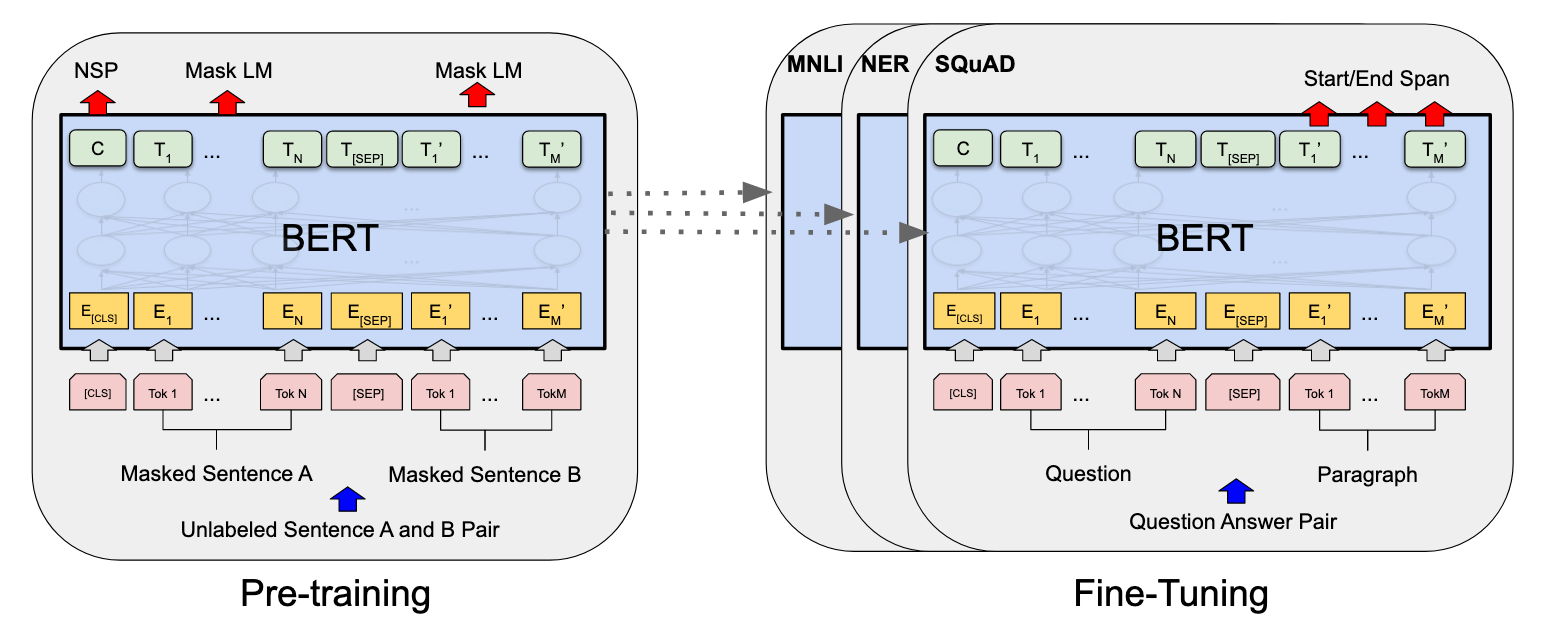
\includegraphics[width=0.95\textwidth]{img/bert.png}}
    \centering
    \caption{Illustration of BERT framework. Figure reprinted from \cite{devlin2018bert}.}
    \label{img:bert}
\end{figure}

Despite it's success in many tasks, especially in natural language understanding (NLU), incorporating BERT in natural language generation (NLG) remains challenging. We conclude the main challenges as three-fold considering that the sequence-to-sequence framework (\cite{sutskever2014sequence}) is the backbone model of generation tasks. On the encoder side, as studied in \cite{Zhu2020IncorporatingBI}, simply initializing the encoder with a pre-trained BERT will actually hurt the performance. One possible explanation could be that training on a complex task with rich resources (e.g., machine translation) leads to the catastrophic forgetting problem (\cite{mccloskey1989catastrophic}) of the pre-trained model. On the decoder side, which can be treated as a conditional language model, it is naturally non-trivial to marry unconditional pre-training with conditional fine-tuning. And the bidirectional nature of BERT also prevents it from being directly applied to common autoregressive text generation. In addition, fine-tuning the full model is parameter inefficient considering the enormous scale of recent pre-trained language models (\cite{ratford2019language}) while being unstable and fragile on small datasets (\cite{Lee2020MixoutER}).

\section{Adapters}
\label{sec:bm_adapters}
Adapters is a light-weight layers which are transplanted between the layers of a pre-trained Transformer network and fine-tuned on the adaptation corpus. Adapters were proposed by \cite{houlsby2019parameter} as an alternative to fine-tuning. There are two different adapter placements as proposed by \cite{bapna2019simple} and \cite{houlsby2019parameter}. The former leverages the adapters by incorporating them in two different parts of the sub-layers. The latter only appends the adapters on top of each layer with layer normalization added within the adapter architecture. As of this writing, there are no direct comparisons between these two techniques. However, the work of \cite{bapna2019simple} is simpler to implement and has been adopted in other works (\cite{pfeiffer2020madx,ruckle2020adapterdrop,pfeiffer2021adapterfusion}).

Following (\cite{pfeiffer2020madx}), adapter is defined with the following formulation

$$A_l(h_l, r_l) = U_l(ReLU(D_l(LA_l))) + r_l $$

$A_l$ is the adapter incorporated at layer $l$, $D_l$ is a down projection layer $D \in R^{h \times d}$ where $h$ is the dimension of the current layer and $d$ is the adapter dimension, $U_l$ is an up projection layer $U \in R^{d \times h}$, and $r_l$ is the residual connection from the previous layer. We can refer to \ref{img:adapters} for illustration of the adapter bottleneck layer and how they are incorporated to the Transformer architecture.

\begin{figure}[h]
    {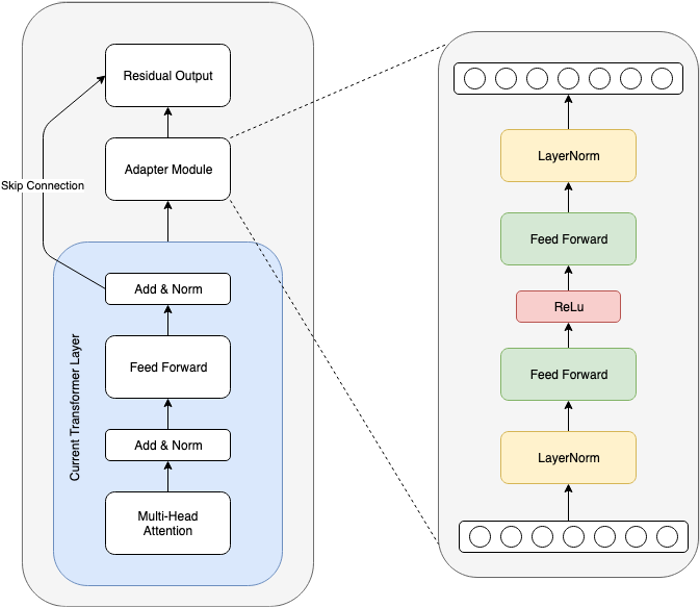
\includegraphics[width=0.75\textwidth]{img/adapter_module.png}}
    \centering
    \caption{Illustration of Adapters.}
    \label{img:adapters}
\end{figure}

Adapters is created to alleviate the problem in fine-tuning. Naive fine-tuning requires training and maintaining a separate model for every language, for every domain. As the number of languages and domains grow, training, maintaining and serving a separate model for every task becomes infeasible. This is further exacerbated by the increasing model capacity of state-of-the-art NMT models (Shazeer et al., 2018; Bapna et al., 2018; Huang et al., 2018); full fine-tuning is just too parameter inefficient. In addition to the growing number of models, fine-tuning requires very careful hyper-parameter tuning (eg. learning rate, regularization knobs etc.) during adaptation, and is prone to rapid over-fitting (Sennrich et al., 2016; Miceli Barone et al., 2017). This sensitivity to hyper-parameters and over-fitting to the adaptation corpus become worse in the setting of high capacity models.

Furthermore, (\cite{han2021robust}) also found that both standard sequential transfer learning and that with task-specific pretraining are unstable in the sense that downstream task performance is subject to considerable fluctuation while the random seed is changed or the number of pretraining and/or fine-tuning iterations is varied even after the training has converged. Some prior works have examined the potential causes of the instability of pretrained language models in transfer learning. Lee et al. (2019) proposed that catastrophic forgetting in sequential transfer learning underlined the instability, while Mosbach et al. (2020) proposed that gradient vanishing in fine-tuning caused it. Pinpointing the cause of transfer learning instability is not the focus of the current work, but our proposed method seems to able to enhance transfer learning on both
aspects. For full illustration, we can refer to \ref{img:adapters_instability}

\begin{figure}[h]
    {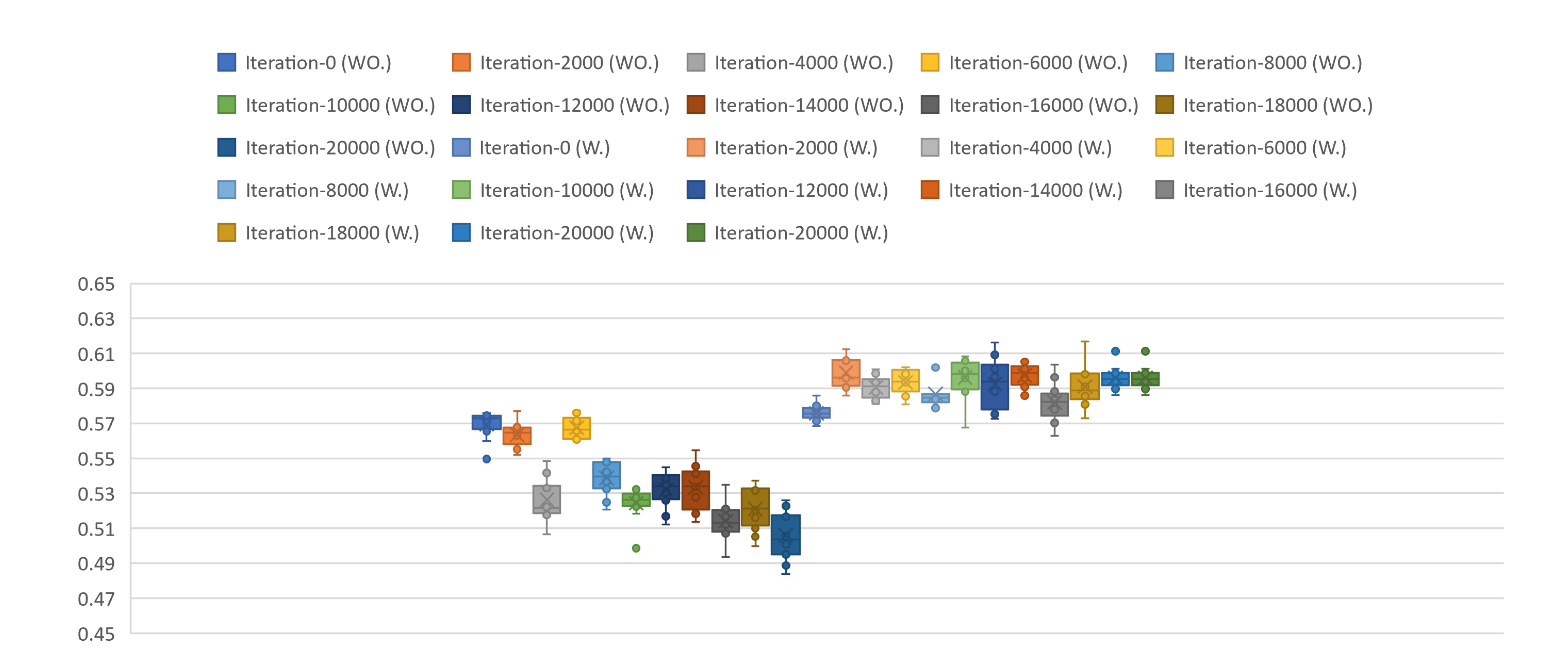
\includegraphics[width=0.95\textwidth]{img/adapters_instability.png}}
    \centering
    \caption{Illustration of Adapters instability. W represents the models that use adapters and WO represents the models that do not use adapters. Figure reprinted from \cite{han2021robust}.}
    \label{img:adapters_instability}
\end{figure}